\chapter{Existence and uniqueness}
When does there exist a unique solution to \eqref{eq: IVP}? There is a standard sufficient condition. The proof by Picard iteration is standard issue mathematics that you must know, and it conveys something important about life.
Suppose for a moment that we wanted to solve instead

\begin{equation}
    \label{eq: no-x ODE}
    \left\{\begin{array}{l}
        x^{\prime}(t)=h(t), \\
        x(0)=x_{0}
        \end{array}\right. 
\end{equation}
where $h$ is some known function. This is easy! The fundamental theorem of calculus guarantees (under mild integrability conditions on $h$ ) the existence of a unique solution as
$$
x(t)=x_{0}+\int_{0}^{t} h(s) d x .
$$
Now suppose we already knew the solution $x(t)$. Then we could define
$$
h(t):=f(x(t), t)
$$
and recover $x(t)$ again as the solution of \eqref{eq: no-x ODE}. We define  $\Phi$ to be the composition of the maps before, so $\Phi$ is a map $x \mapsto \Phi[x]$ from functions to functions defined by
$$
\Phi[x](t)=x_{0}+\int_{0}^{t} f(x(s), s) d x
$$
The self-consistency discussion is precisely saying that we are looking for fixed points of this map, i.e., $x$ such that $\Phi[x]=x$.


%────────────────────────────────────────
\begin{definition}
[Function space]
\label{def: Function space}
Let $C\left([0, T] ; \mathbb{R}^{d}\right)$ denote the space of continuous functions $[0, T] \rightarrow \mathbb{R}^{d}$. Let $\|\cdot\|_{\infty}$ denote the uniform (or sup) norm on $C\left([0, T] ; \mathbb{R}^{d}\right)$, defined by
$$
\|g\|_{\infty}=\sup \{|g(t)|: t \in[0, T]\} .
$$
Here $\mid \cdot$ denotes the Euclidean norm on $\mathbb{R}^{d}$, which will be our convention throughout.
\end{definition}
%────────────────────────────────────────


%────────────────────────────────────────
\begin{remark}
    Recall that $C\left([0, T] ; \mathbb{R}^{d}\right)$ is a Banach space with respect to the uniform norm, i.e., it is a complete metric space with respect to the metric $d(g, h)=\|g-h\|_{\infty}$.
\end{remark}
%────────────────────────────────────────

\section{Banach fixed point theorem}
The key theorem for proving the existence of fixed points is the Banach fixed point theorem. Note that the proof is constructive via an iterative scheme, which even comes with a rate of convergence.


%────────────────────────────────────────
\begin{theorem}
[Banach fixed point ]
\label{thm: Banach fixed point }
 Let $X$ denote a complete metric space with metric $d$. Suppose that $\Phi: X \rightarrow X$ is a contraction map, i.e., there exists $\alpha \in[0,1)$ such that
$$
d(\Phi(x), \Phi(y)) \leq \alpha d(x, y)
$$
for all $x, y \in X$. Then there exists a unique fixed point for the map $\Phi$, i.e., a unique $x^{\star}$ such that $\Phi\left(x^{\star}\right)=x^{\star}$. Moreover, for any $x \in X$, if we define the sequence $\left\{x_{k}\right\}_{k=0}^{\infty}$ via $x_{0}=x$ and $x_{k}=\Phi\left(x_{k-1}\right)$ for all $k \geq 1$, then $\lim _{k \rightarrow \infty} x_{k}=x^{\star}$. In other words, the result of repeated application of $\Phi$ converges to $x^{\star}$ for arbitrary initial input.
\end{theorem}
%────────────────────────────────────────

%────────────────────────────────────────
\begin{remark}
In fact, the proof recovers a convergence rate for the limit $x_{k} \rightarrow x^{\star}$. To wit, we have $d\left(x_{k}, x^{\star}\right)=O\left(\alpha^{k}\right)$
\end{remark}
%────────────────────────────────────────

\section{Picard-Lindel\"of theorem}
The key sufficient condition establishing existence and uniqueness of solutions of \eqref{eq: ODE} phrased in terms of Lipschitz functions.


%────────────────────────────────────────
\begin{definition}
[Lipschitz]
\label{def: Lipschitz}
A function $f: \mathbb{R}^{n} \rightarrow \mathbb{R}$ is Lipschitz (or Lipschitz continuous) if there exists $L \geq 0$ such that $|f(u)-f(v)| \leq L|u-v|$ for all $u, v \in \mathbb{R}^{n}$. In this case we can say more specifically that $f$ is $L$-Lipschitz, and $L$ is a Lipschitz constant. 
\end{definition}
%────────────────────────────────────────


%────────────────────────────────────────
\begin{theorem}
[Picard-Lindel\"of]
\label{thm: Picard-Lindelof}
Suppose that $f$ is Lipschitz. Then the system \eqref{eq: IVP} i.e.,
$$
\left\{\begin{array}{l}
x^{\prime}(t)=f(x(t), t), \\
x(0)=x_{0},
\end{array}\right.
$$
admits a unique solution on $[0, T]$ for any $T>0$.
\end{theorem}
%────────────────────────────────────────
%────────────────────────────────────────
\begin{proof}
Note that 
\[
    \begin{aligned}
        \|\Phi[x]-\Phi[y]\|_{\infty} & =\sup _{t \in[0, T]}\left\{\left|\int_0^t f(x(s), s)-f(y(s), s) d x\right|\right\} \\
        & \leq \sup _{t \in[0, T]}\left\{\int_0^t|f(x(s), s)-f(y(s), s)| d x\right\} \\
        & \leq \sup _{t \in[0, T]}\left\{L \int_0^t|x(s)-y(s)| d x\right\} \\
        & \leq \sup _{t \in[0, T]}\left\{L \int_0^t\|x-y\|_{\infty} d x\right\} \\
        & \leq L T\|x-y\|_{\infty} .
        \end{aligned}
\]
If we have $ LT<1 $, then we have a contraction map. Unfortunately this cannot be guaranteed a priori.

We sidestep the difficulty in the following way. Let $h=T / N$, where $N$ is sufficiently large such that $L h<1$, and consider dividing the interval $[0, T]$ into the $N$ subintervals
$$
I_0:=[0, h], I_1:=[h, 2 h], \ldots, I_{N-1}:=[(N-1) h, T] .
$$
We are going to construct a solution for (1.1) on each of these intervals individually and then argue that together they constitute a solution on $[0, T]$.
Indeed let us first define $\Phi_0: C\left(I_0 ; \mathbb{R}^d\right) \rightarrow C\left(I_0 ; \mathbb{R}^d\right)$ via
$$
\Phi_0[y](t)=x_0+\int_0^h f(y(s), s) d s .
$$
Our preceding calculation ensures that $\Phi_0$ is a contraction mapping, hence admits a unique fixed point in $C\left(I_0 ; \mathbb{R}^d\right)$, which is therefore the unique solution of \eqref{eq: IVP} on $I_0$. As this solution is continuous up to the boundary of $[0, h]$, the final state $x_1:=x(h)$ is well-defined.

Then we can consider $x_1$ as the initial condition of (1.1) on the interval $[h, 2 h]$. By shifting the time variable appropriately, the same argument suggests that we can extend $x$ continuously to the interval $[0,2 h]$ such that $x$ solves \eqref{eq: IVP} on both $[0, h]$ and $[h, 2 h]$, and we define $x_2:=x(2 h)$.

More concretely, given the preceding final state $x_n$, we inductively define $\Phi_n: C\left(I_n ; \mathbb{R}^d\right) \rightarrow$ $C\left(I_n ; \mathbb{R}^d\right)$ via
$$
\Phi_n[y](t)=x_n+\int_{n h}^t f(y(s), s) d s
$$
This is a contraction mapping, and we can extend $x$ continuously to $[0,(n+1) h]$ by appending its unique fixed point. Then we define $x_{n+1}=x((n+1) h)$ to complete the inductive procedure.

In summary the construction yields $x \in C\left([0, T] ; \mathbb{R}^d\right)$ with $x_n=x(n h)$, solving \eqref{eq: IVP} on each of the individual subintervals $I_n, n=0, \ldots, N-1$ in the sense that the restriction $\left.x\right|_{I_n}$ is the unique fixed point of $\Phi_n$ for each $n$. Then this solution must be unique on $ [0,T] $. 
\end{proof}
%────────────────────────────────────────

%────────────────────────────────────────
\begin{note}
Note that the most famous counterexample to global-in-time existence, the scalar equation $x^{\prime}(t)=x(t)^2$, does not satisfy the Lipschitz condition. Solutions of this ODE blow up in finite time, as can be checked by direct solution via separation of variables.
\end{note}
%────────────────────────────────────────

\section{Significance of Lipschitz constant} 
The Lipschitz constant measures how much $f(u, t)$ changes if we perturb $u$ (at some fixed time $t)$. Since $f(u, t)=u^{\prime}(t)$, the slope of the line tangent to the solution curve through the value $u$, this indicates how the slope of the solution curve will vary if we perturb $u$. The significance of this is best seen through some examples. 


%────────────────────────────────────────
\begin{example}
\label{eg: Lip Integral}
Consider $ u^\prime (t) = g(t) $ and the solution is 
\[
    u(t) = u(t_0) + \int_{t_0}^{t} g(\tau) \, d\tau.  
\]
The Lipschitz constant is $ L=0 $. And we have the following figure:
%────────────────────────────────────────
\begin{figure}[H]
    \centering
    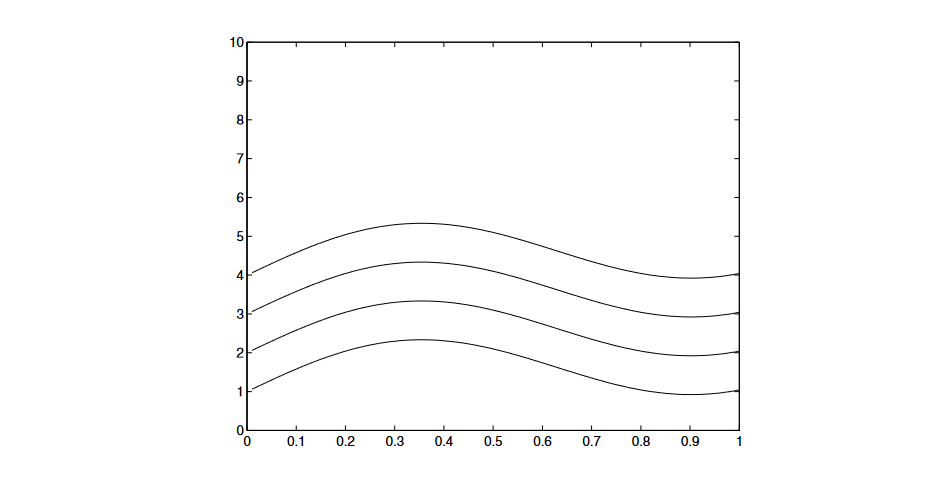
\includegraphics[width=0.6\textwidth]{figures/2-1.png}
\end{figure}
%────────────────────────────────────────
Note that all these curves are ``parallel'', since the tangent line at any particular time only depends on $ t $. 
\end{example}
%────────────────────────────────────────


%────────────────────────────────────────
\begin{example}
\label{eg: Lip expo}
Consider $ u^\prime (t) = \lambda u(t) $ with $ \lambda  $ constant and $ L= |\lambda | $. Then, $ u(t) = u(0) \exp (\lambda t) $. Then, we have 
%────────────────────────────────────────
\begin{figure}[H]
    \centering
    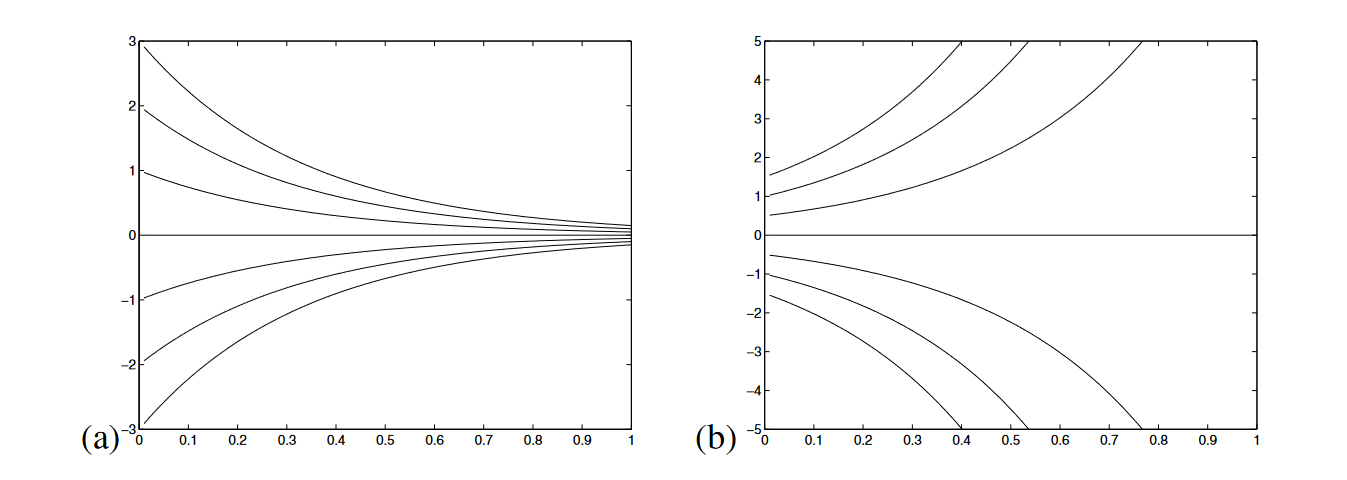
\includegraphics[width=0.8\textwidth]{figures/2-2.png}
\end{figure}
%────────────────────────────────────────
Here $ \lambda =-3 $ for  (a)  and $ \lambda =3 $ for (b). Here the slope of the solution curve does vary depending on $u$. The variation in the slope with $u$ (at fixed $t$ ) gives an indication of how rapidly the solution curves are converging toward one another (in the case $\lambda<0$ ) or diverging away from one another (in the case $\lambda>0$ ). If the magnitude of $\lambda$ were increased, the convergence or divergence would clearly be more rapid.
\end{example}
%────────────────────────────────────────

However, rapidly converging solution curves can also give serious numerical difficulties, which one might not expect at first glance. This is discussed in detail later, which covers stiff equations.

One should also keep in mind that a small value of the Lipschitz constant does not necessarily mean that two solution curves starting close together will stay close together forever.


%────────────────────────────────────────
\begin{example}
[Pendulum problem]
\label{eg: Pendulum problem}
Consider the pendulum problem: 
\[
    \theta ^{\prime \prime}(t) = -\sin(\theta (t)), 
\]
which can be rewritten as a first order system of two equations by introducing $ v(t) = \theta ^\prime (t) $: 
\[
    u=\left[\begin{array}{l}
        \theta \\
        v
        \end{array}\right], \quad \frac{d}{d t}\left[\begin{array}{l}
        \theta \\
        v
        \end{array}\right]=\left[\begin{array}{c}
        v \\
        -\sin (\theta)
        \end{array}\right] .
\]
Consider the max-norm. We have
$$
\left\|u-u^*\right\|_{\infty}=\max \left(\left|\theta-\theta^*\right|,\left|v-v^*\right|\right)
$$
and
$$
\left\|f(u)-f\left(u^*\right)\right\|_{\infty}=\max \left(\left|v-v^*\right|,\left|\sin (\theta)-\sin \left(\theta^*\right)\right|\right) .
$$
To bound $\left\|f(u)-f\left(u^*\right)\right\|_{\infty}$, first note that $\left|v-v^*\right| \leq\left\|u-u^*\right\|_{\infty}$. We also have
$$
\left|\sin (\theta)-\sin \left(\theta^*\right)\right| \leq\left|\theta-\theta^*\right| \leq\left\|u-u^*\right\|_{\infty}
$$
since the derivative of $\sin (\theta)$ is bounded by 1 . So we have Lipschitz continuity with $L=1$ :
$$
\left\|f(u)-f\left(u^*\right)\right\|_{\infty} \leq\left\|u-u^*\right\|_{\infty} .
$$

Consider two solutions to the pendulum problem  one with initial data
$$
\theta_1(0)=\pi-\epsilon, \quad v_1(0)=0,
$$
and the other with $$
\theta_2(0)=\pi+\epsilon, \quad v_2(0)=0 .
$$
The Lipschitz constant is 1 and the data differ by $2 \epsilon$, which can be arbitrarily small, and yet the solutions eventually diverge dramatically, as Solution 1 falls toward $\theta=0$, while in Solution 2 the pendulum falls the other way, toward $\theta=2 \pi$.

In this case the IVP is very ill conditioned: small changes in the data can lead to order 1 changes in the solution. As always in numerical analysis, the solution of ill-conditioned problems can be very hard to compute accurately.
\end{example}
%────────────────────────────────────────